

\lstset{
 columns=fixed,       
 numbers=left,                                        % 在左侧显示行号
 numberstyle=\tiny\color{gray},                       % 设定行号格式
 frame=none,                                          % 不显示背景边框
 backgroundcolor=\color[RGB]{245,245,244},            % 设定背景颜色
 keywordstyle=\color[RGB]{40,40,255},                 % 设定关键字颜色
 numberstyle=\footnotesize\color{darkgray},           
 commentstyle=\it\color[RGB]{0,96,96},                % 设置代码注释的格式
 stringstyle=\rmfamily\slshape\color[RGB]{128,0,0},   % 设置字符串格式
 showstringspaces=false,                              % 不显示字符串中的空格
 language=c,                                        % 设置语言
}


\chapter{模块验证与实验}
基于NB-IOT的中断应用大致分为4类,分别是固定上报类,固定控制类,移动上报类和移动控制类。不同类别的应用因为数据的实时性、数据量、部署环境等的不同,对网络以及电源的需求也不同。例如对于固定控制类,由于设备部署位置固定,常有外部电源支持,需要较强的实时性,所以对功耗需求不高,需要模块时刻保持在线状态。接下来将以一个固定上报类终端对bc35g模块进行验证。
\section{华为云平台应用开发}
华为 OceanConnect物联网平台作为一个连接业务应用和物联网设备的中间层,提供了海量设备接入管理,屏蔽复杂的设备接口,可以快速构筑物联网应用。
%\begin{figure}[h]
%    \floatcontinue
%	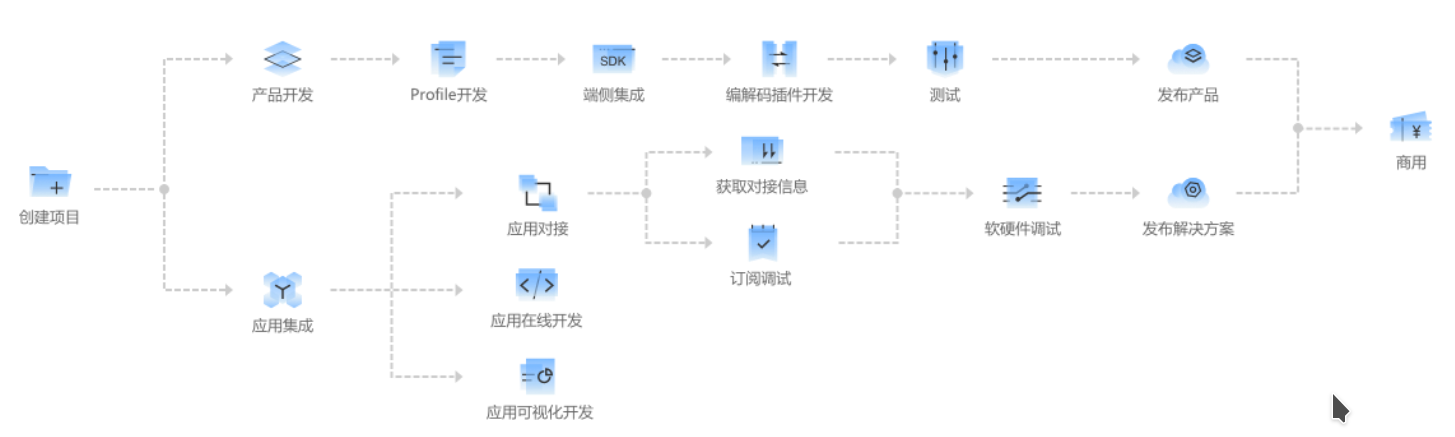
\includegraphics[width=20cm]{oc流程.png}
%	\caption{oc流程}
%	\label{oc流程}
%\end{figure}

\subsection{定义产品}
产品是指一类具备相同能力和特征的设备,一个产品包含产品模型、编解码插件等资源。选用CoAp协议,由于使用JSON的数据格式对能耗消耗太大,不适用于物联网设备,所以选用二进制码流的数据格式,通过开发编解码插件解析。
\begin{figure}[H]
    \centering
	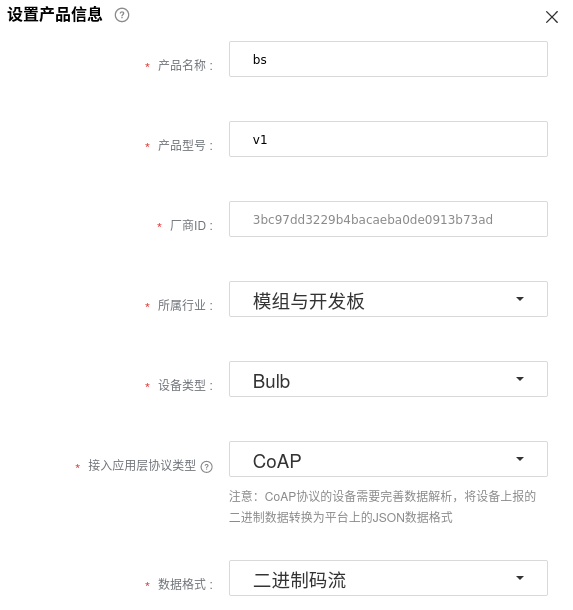
\includegraphics[width=9cm]{oc产品.png}
	\caption{oc产品定义}
	\label{oc产品}
\end{figure}


\subsection{定义profile与编解码插件}
profile是描述产品设备信息的文件,定义了设备与应用服务器交互的字段及格式。其主要包含产品信息、服务能力以及维护能力。以控制开发板LED灯相关的profile信息为例,定义profile如下:
\begin{table}[h]
\caption{profile格式}
\begin{tabular}{|c|c|c|c|c|}
\toprule
\multicolumn{5}{|l|}{属性列表} \\
\hline
属性名称 & 类型 & 取值 & \multicolumn{2}{|c|}{描述}  \\
\hline
status & int & 0~1 & \multicolumn{2}{|l|}{0:灯关闭 1:灯开启} \\
\toprule
\multicolumn{5}{|l|}{命令列表} \\
\hline\
命令名称 & 字段属性 & 字段名 & 取值 & 描述\\
\hline
\multirow{3}{*}{led} & 请求 & num & 1-2 & led 编号 \\
\cmidrule{2-5}
                     & 请求 & status & 0-1 & led状态 \\
\cmidrule{2-5}
                     & 响应 & result & 0-1 & 执行命令结果 \\
\hline
\multirow{2}{*}{beep} & 请求 & status & 0-1 & 蜂鸣器状态 \\
\cmidrule{2-5}
                      & 响应 & result & 0-1 & 执行命令结果 \\
\hline
\multirow{2}{*}{query} & 请求 & resource & 1-3 & 资源编号 \\
\cmidrule{2-5}
                      & 响应 & result & 0-1 & 执行命令结果 \\
\bottomrule
\end{tabular}
\label{tablea}
\end{table}

二进制数据格式需要编解码插件才能解析,在oc平台上设置好profile 文件后,将相应属性值与消息模板中的字段相连接,oc平台将会自动生成编解码器。

\subsection{接入设备}
通过串口连接设备,使用AT+CSGB=1命令查询设备IMEI号,在oc平台上增加设备,并从oc平台获取CoAP接入地址,填入stm32代码,华为云平台上的设置就完成了。(TODO:补图)


\section{stm32终端开发}
stm32终端选择一块搭载stm32f103zet的开发板,板载4组串口,第一组可用于USB通信。本次验证使用到其中第二组串口,对应引脚为PA2和PA3。使用无源蜂鸣器及一组LED灯,作为控制量,对应引脚为PB8,PB5,PE5。


\subsection{串口DMA通信}

stm32开发板控制bc35g模块是通过串口的方式,bc35g串口比特率为9600。由于HAL库函数仅提供接受固定长度数据的封装,为了接受变长的串口数据,可以有以下几种方式:

BC35G模块串口传输数据以'lr cr'为分隔符,以软件的方式,设置超时接收固定长度并以'lr cr'分割,放入缓冲区中。由于模块涉及网络操作等原因,不同AT指令的响应时间有很大差距,所以超时时间不好确定,同时由于MCU等待模块输入,对效率影响较大。

利用定时器中断方式可以超时时间设置的问题。一个字节的数据有 起始位+数据+结束位共10位,在模块串口比特率为9600的情况下,传输一个字节需要104us。同时由于两组数据之间需要间隔3.5字符,可以设置定时器中断为5ms。在串口接受中断服务函数中开启定时器中断,每接受一个字符则重置定时器,当定时器超时时可以认为一组数据接受完毕,在定时器中断函数中将接收到的数据放入缓存中。但是由于是一字节一字节接受,而且MCU仍然参与接受过程,所以效率仍有提升必要。

为了进一步提升效率,可以使用DMA方式接受数据。为了区分两组数据,开启总线空闲中断,在总线空闲中断中标记数据就绪。这种方式能获得更好的效率。

\begin{lstlisting}

/* main.c
* 使能串口2的总线空闲中断
*/
__HAL_UART_ENABLE_IT(&huart2,UART_IT_IDLE);

/* uart.c
* 检测空闲中断,标记数据可用,并重新开启中断用于下次接收
*/

uint8_t UART2DATAREADY = 0;
uint8_t UART2RXBUFFER[UART_BUFFER_SIZE];

void USER_UART_IRQHandler(UART_HandleTypeDef *huart) {
    if (huart == &huart2) {
        if (RESET != __HAL_UART_GET_FLAG(&huart2, 
                UART_FLAG_IDLE)) {
            __HAL_UART_CLEAR_IDLEFLAG(&huart2);
            HAL_UART_DMAStop(&huart2);
            UART2DATAREADY = UART_BUFFER_SIZE - 
            __HAL_DMA_GET_COUNTER(&hdma_usart2_rx);
        }
    }
}

/* nbiot.c
* 封装AT指令执行模块,接收串口回传数据
*/
void NBCommand(uint8_t *com, uint8_t com_size, 
                char *res, uint8_t *res_size) {
    HAL_UART_Transmit(&huart2, com, com_size - 1, 0xfff);
    HAL_UART_Receive_DMA(&huart2, 
                        UART2RXBUFFER, 
                        UART_BUFFER_SIZE);
    while (!UART2DATAREADY) {
        HAL_Delay(50);
    }
    memcpy(res, UART2RXBUFFER, UART2DATAREADY);
    *res_size = UART2DATAREADY;
    UART2DATAREADY = 0;
}

\end{lstlisting}

\subsection{入网初始化}
bc35g模块入网操作流程如图(TODO:临时图)

\begin{figure}[H]
    \centering
	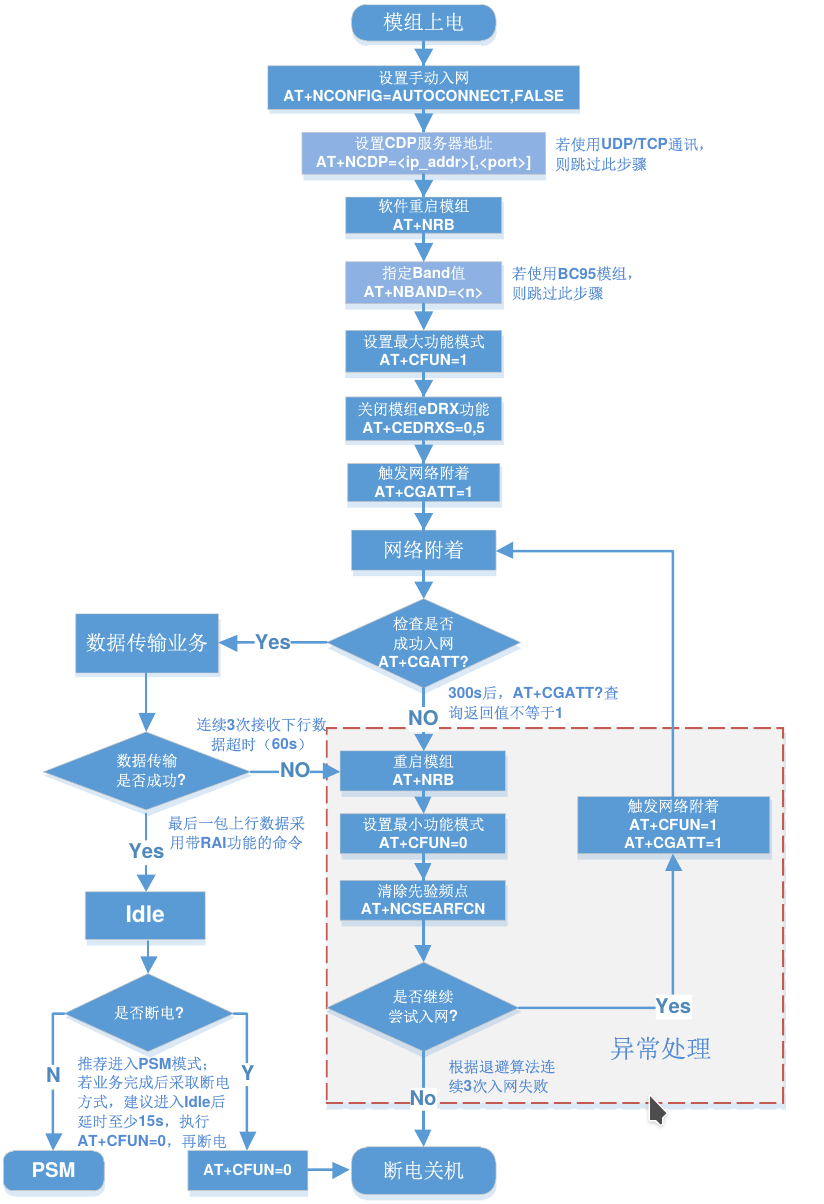
\includegraphics[width=10cm]{模块入网操作.png}
	\caption{模块入网}
	\label{模块入网}
\end{figure}

\begin{lstlisting}

/*
* nbiot.c
*/
uint8_t (*InitProc[])() ={
        __NB_MODULE_STATUS,
        __NB_SIGNAL_QUALITY,
        __NB_Manual,
        __NB_SetCDP,
        __NB_ModReboot,
        __NB_SetBand,
        __NB_SetBand,
        __NB_OpenCFun,
        __NB_EdrxOff,
        __NB_PSMOff,
        __NB_NETATT,
};

uint8_t NBInit() {
    unsigned int it = 0;
    for (it = 0; it < sizeof InitProc; it++) {
        if (!InitProc[it]()) {
            NBERROR(it);
        }
    }
    return 1;
}
\end{lstlisting}

\subsection{模组通信}

NBIOT模块使用 AT+NMGS命令发送数据

\subsection{退网关机}
\begin{lstlisting}

\end{lstlisting}


\section{验证过程以及结论}

\section{本章小结}
